% ============================================
% SECTION 1: Introduction
% ============================================
\section{Introdução}

\begin{frame}{Contexto - Documentos e Compliance}
\begin{itemize}
    \item Ambiente Bancário
    \item Classificação de documentos
    \item Exemplos:
    % \begin{itemize}
    %     \item Carteira de identidade
    %     \item Carteira de habilitação
    %     \item Recibos
    %     \item Contratos
    % \end{itemize}
    \begin{center}
    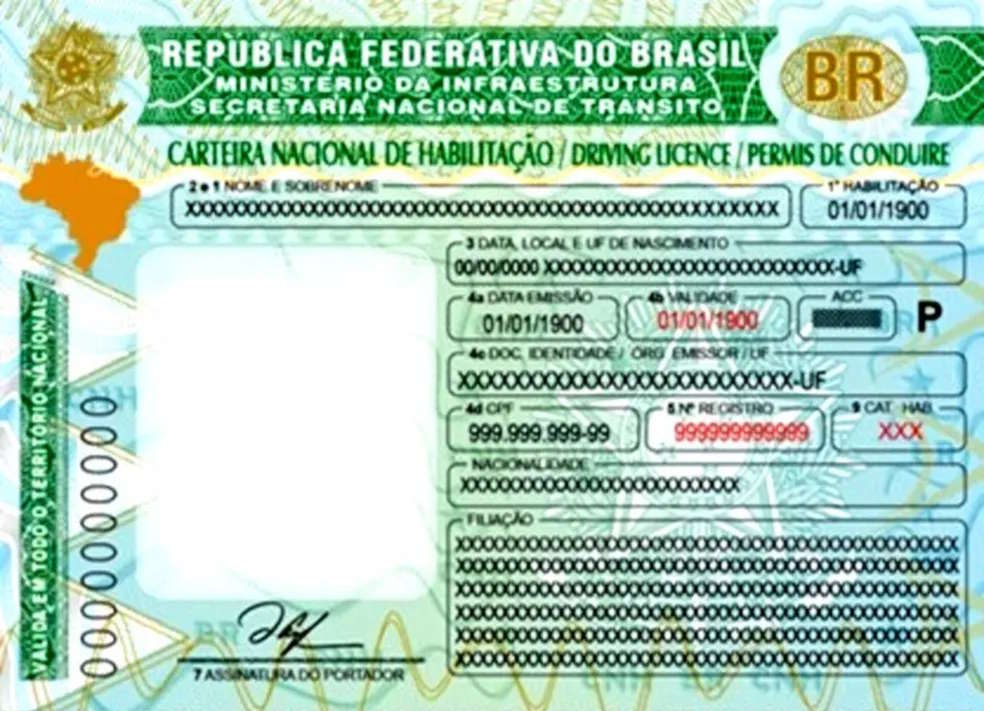
\includegraphics[width=0.27\textwidth]{images-apresentacao/CNH_EXEMPLO.jpg}
    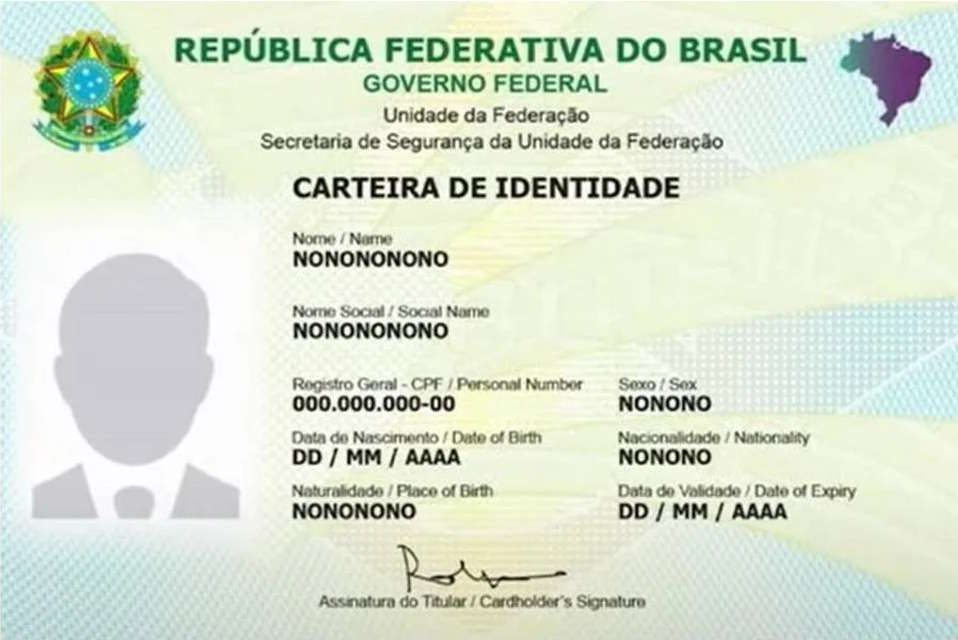
\includegraphics[width=0.29\textwidth]{images-apresentacao/CIN_EXEMPLO.jpg}
    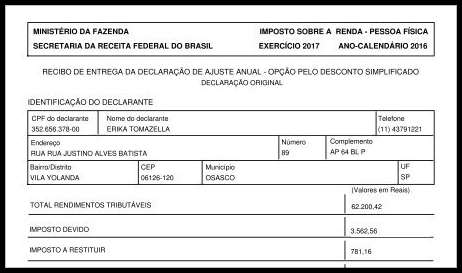
\includegraphics[width=0.33\textwidth]{images-apresentacao/IRPF_EXEMPLO.jpg}
\end{center}
\end{itemize}
\end{frame}

\begin{frame}{Evolução dos Documentos}
\begin{center}
\begin{tikzpicture}
    \node (antiga) at (0,0) {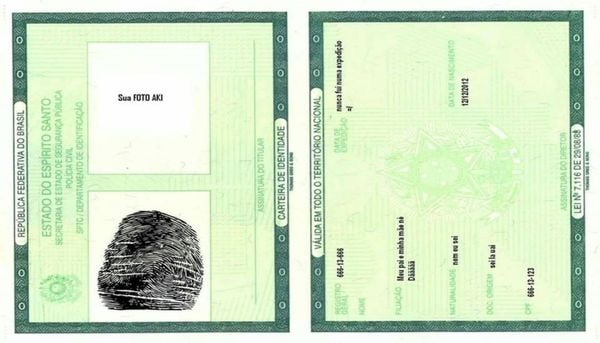
\includegraphics[width=0.40\textwidth]{images-apresentacao/carteira_de_identidade_antiga.jpg}};
    \node (nova) at (7,0) {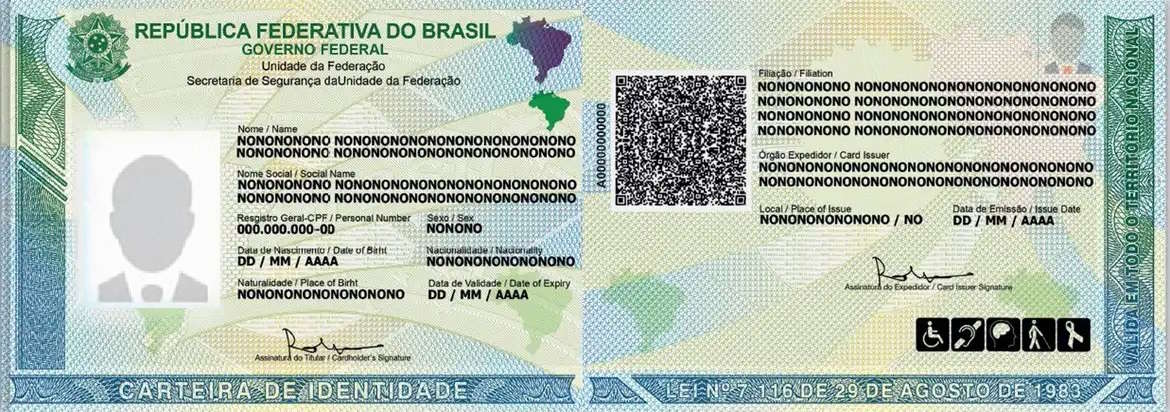
\includegraphics[width=0.40\textwidth]{images-apresentacao/carteira_de_identidade_nova.jpg}};
    \draw[->, line width=3pt, color=UnBBlue] (antiga.east) -- (nova.west);
\end{tikzpicture}
\end{center}
\end{frame}

\begin{frame}{Solução}
    \begin{center}
        {\Huge \textbf{Zero-Shot Learning}}\\ \vspace{0.5cm}
        Permite que o modelo reconheça elementos de\\ classes nunca vistas no treinamento
    \end{center}
\end{frame}

\begin{frame}{Sobre a Pesquisa}
\begin{block}{Contribuições}
    \begin{enumerate}
        \item \textbf{Novo dataset LA-CDIP}
        \begin{itemize}
            \item Classificação ZSL
            \item Derivado do RVL-CDIP
        \end{itemize}
        
        \item \textbf{Abordagem de Visual Document Matching (VDM)}
        \begin{itemize}
            \item Similaridade de documentos
            \item Metric Learning
            \item Generalização Zero-Shot
        \end{itemize}
        
        \item \textbf{Avaliação sistemática}
        \begin{itemize}
            \item Benchmark extensivo
        \end{itemize}
    \end{enumerate}
\end{block}
\end{frame}
